%%%%%%%%%%%%%%%%%%%%%%%%%%%%%%%%%%%%%%%%%
% Thin Sectioned Essay
% LaTeX Template
% Version 1.0 (3/8/13)
%
% This template has been downloaded from:
% http://www.LaTeXTemplates.com
%
% Original Author:
% Nicolas Diaz (nsdiaz@uc.cl) with extensive modifications by:
% Vel (vel@latextemplates.com)
%
% License:
% CC BY-NC-SA 3.0 (http://creativecommons.org/licenses/by-nc-sa/3.0/)
%
%%%%%%%%%%%%%%%%%%%%%%%%%%%%%%%%%%%%%%%%%

%----------------------------------------------------------------------------------------
%	PACKAGES AND OTHER DOCUMENT CONFIGURATIONS
%----------------------------------------------------------------------------------------

\documentclass[a4paper, 11pt]{article} % Font size (can be 10pt, 11pt or 12pt) and paper size (remove a4paper for US letter paper)

\usepackage[protrusion=true,expansion=true]{microtype} % Better typography
\usepackage{graphicx} % Required for including pictures
\usepackage{wrapfig} % Allows in-line images

\usepackage{mathpazo} % Use the Palatino font
\usepackage[T1]{fontenc} % Required for accented characters
%\usepackage[backend=bibtex,style=verbose-trad2]{biblatex}
\usepackage{hyperref}
\usepackage{longtable}
\usepackage{array}
\usepackage{multirow}
\usepackage[utf8]{inputenc}
\usepackage{subcaption}
\usepackage[font=small]{caption}
\usepackage{units}
\usepackage{relsize}
\usepackage{gensymb}
\usepackage{textcomp}
\usepackage{lipsum}

\linespread{1.05} % Change line spacing here, Palatino benefits from a slight increase by default

\makeatletter
\renewcommand{\refname}{Bibliografie}
\renewcommand{\@listI}{\itemsep=0pt} % Reduce the space between items in the itemize and enumerate environments and the bibliography

\renewcommand{\maketitle}{ % Customize the title - do not edit title and author name here, see the TITLE block below
	\begin{flushright} % Right align
		{\LARGE\@title} % Increase the font size of the title
		
		\vspace{50pt} % Some vertical space between the title and author name
		
		{\large\@author} % Author name
		\\\@date % Date
		
		\vspace{40pt} % Some vertical space between the author block and abstract
	\end{flushright}
}

%----------------------------------------------------------------------------------------
%	TITLE
%----------------------------------------------------------------------------------------

\title{\textbf{Ontwerpverslag}\\ % Title
	De implementatie van een koolstofmonoxidesensor} % Subtitle

\author{\textsc{R. Bolding} % Author
	\\{\textit{Amsterdam University of Applied Sciences\\ 
			HvA\\
			Sensor Netwerken: groep 5\\
			Studentnummer: 500757732}}} % Institution

\date{9 december, 2019} % Date

%----------------------------------------------------------------------------------------
\begin{document}
	\captionsetup[figure]{labelfont={bf},name={Fig},labelsep=period}
	\captionsetup{justification=centering}
	\renewcommand{\contentsname}{Inhoudsopgave}
	\def\textsubscript#1{\ensuremath{_{\mbox{\textscale{.6}{#1}}}}}
	\hypersetup{hidelinks=true}
	\maketitle % Print the title section
	
	%----------------------------------------------------------------------------------------
	%	ABSTRACT AND KEYWORDS
	%----------------------------------------------------------------------------------------
	
	%\renewcommand{\abstractname}{Summary} % Uncomment to change the name of the abstract to something else
	
	
	\vspace{10pt} % Some vertical space between the abstract and first section
	
	%----------------------------------------------------------------------------------------
	%	ESSAY BODY
	%-----------------------------------------------
	\newpage
	\tableofcontents
	\newpage
	\section{Specificaties sensormodule} \label{sec::specificaties}
	Zie tabel \ref{tab::specs} voor een overzicht van de specificaties van de sensormodule.
	\begin{center}
		\begin{tabular}{ | m{5cm} | m{5cm}| } 
			\hline
			\multicolumn{2}{|c|}{Specificaties voor de implementatie van de CO sensor} \\
			\hline
			Meetbereik a: & 0 - 200 \textit{ppm} \\
			\hline
			detectie limiet:  & <2 \textit{ppm}
			\\ 
			\hline
			detectie resolutie: & 2 \textit{ppm} 
			\\ 
			\hline
			responstijd: & < 3 minuut
			\\ 
			\hline
			Voed spanning: & min: 2,7V max: 3,3V
			\\ 
			\hline
			Maximaal vermogen: & 1 mW
			\\
			\hline
			Output gevoeligheid: & 1mV/\textit{ppm}
			\\
			\hline
		\end{tabular}\label{tab::specs}
	\end{center}

	\section{De complete sensornode} \label{sec::sensornode}
	De sensornode is gehele systeem. Hieronder vallen de sensoren met de nodige signaal verwerking, de omzetting van de analoge signalen naar het digitale domein, de compensatie van de signalen en het netwerkalgoritme in de software van de Xmega. Zie figuur \ref{fig::sensorNode_dia} voor een visueel overzicht van de sensornode.
	\begin{figure}[h!]
		\centering
		\hspace*{-4cm} 
		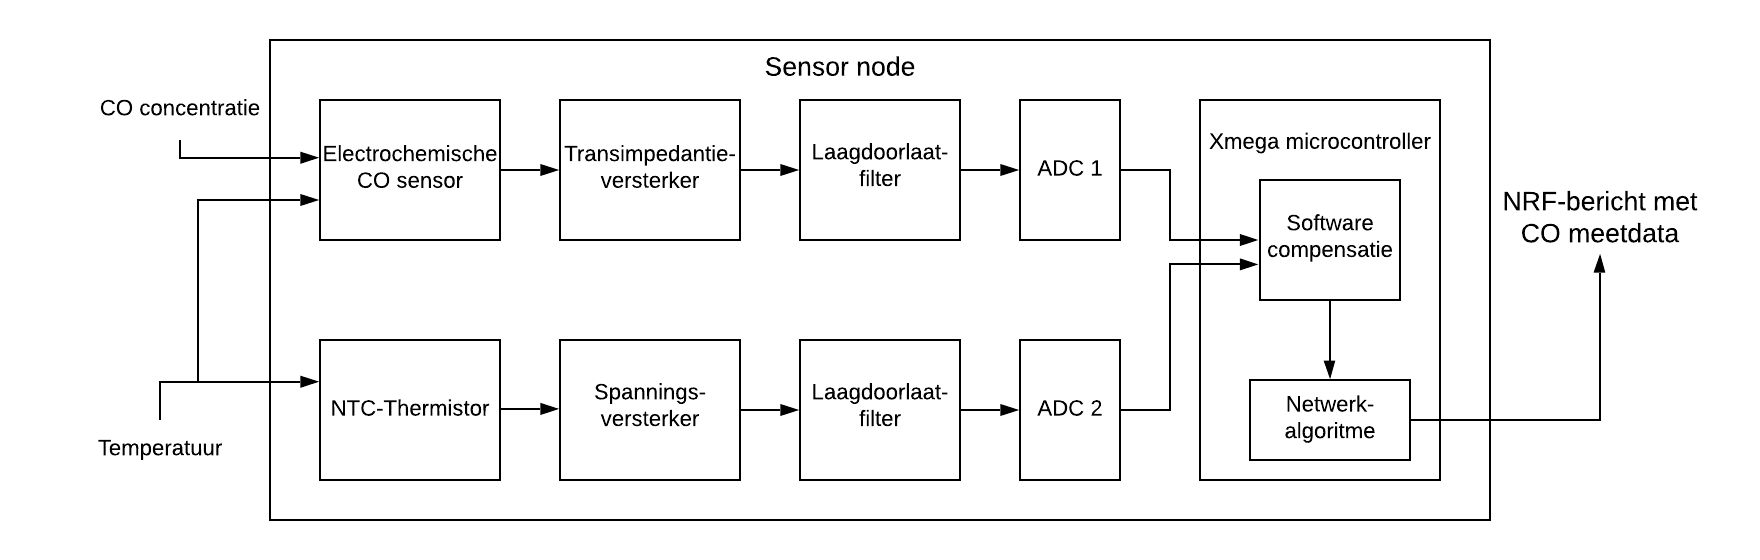
\includegraphics[width=1.7\linewidth]{../Media/sensorNode_dia.png}
		\caption{Blokdiagram van het complete systeem van de sensornode}
		\label{fig::sensorNode_dia}
	\end{figure}
	\newpage
	\section{Elektrochemische CO-sensor } \label{sec::EG_CO_sensor}
	In dit hoofdstuk wordt er besproken wat er nodig is om de elektrochemische CO-sensor te laten werken en wat de nodige signaalverwerking is om de sensor correct uit te kunnen lezen. Als elektrochemische CO-gassensor is er gekozen voor de \textit{3SP\_CO\_1000 package 110-102}.

	\subsection{Potentiostat} \label{subsec::potentiostat}
	De gekozen elektrochemische CO-gassensor heeft 3 elektroden: een \textit{sensing elektrode} (SE), een \textit{counter elektrode} (CE) en een \textit{referentie elektrode} (RE) \cite{datasheet sensor}.
	\\ Kort samengevat: bij de SE vindt er een reactie met het doelgas (CO) plaats, bij de CE volgt een reactie op het resultaat van de reactie bij de SE en de RE zorgt ervoor dat er geen spanningsverschil ontstaat tijdens de reacties. Hiervoor moet de RE verbonden zijn met de SE. Om het spanningsverschil tussen de RE en de SE gelijk te houden is er een potentiostat schakeling nodig \cite{datasheet sensor}. Afhankelijk van het type sensor is er een bepaalde bias-spanning nodig tussen de RE en de SE \cite{SGX Application note}, in het geval van de \textit{3SP\_CO\_1000 package 110-102} is deze 0V \cite{datasheet sensor}.
	\begin{figure}[h!]
		\centering
		\hspace*{-3cm} 
		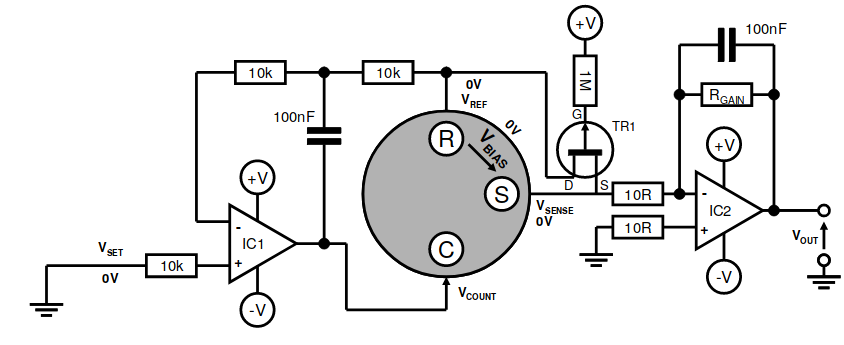
\includegraphics[width=1.4\linewidth]{../Media/unbiasedSensorCircuit.png}
		\caption{Voorbeeld van een een potetiostat schakeling met 0V bias spanning en een transimpendantieversterker \cite{SGX Application note}}
		\label{fig::EG_schakeling}
	\end{figure}
	\newpage
	OP-AMP IC1 behoudt het potentiaal van RE, V{\small ref} en past het geschikte potentiaal V{\small count} op CE om V{\small ref} gelijk te houden aan V{\small set}. Dit potentiaal zal veranderen omdat wanneer de CO-concentratie verandert omdat het stroom levert aan de CE om de outputstroom van de SE te balanceren. Om er voor te zorgen dat het potentiaalverschil zo nauwkeurig mogelijk bepaald kan worden door de potentiostat, moet er voor IC1 een OP-AMP met een lage offset spanning gekozen worden.\\
	TR1 is een \textit{p-channel FET}, deze zorgt ervoor dat het spanningsverschil tussen de RE en SE 0V blijft wanneer er geen voeding aanwezig is. Een lage spanning op de \textit{gate} van de \textit{FET} zorgt er voor dat deze gaat geleiden en daarvoor V{\small ref} = V{\small set} blijft \cite{SGX Application note}.
	
	\subsection{Transimpedantieversterker} \label{subsec::transimpedantieversterker}
	De output van de elektrochemische CO-gassensor is een stroom. De waarde die van een ADC uitgelezen kan worden is afhankelijk van de spanning. De output zal dus moeten worden omgezet naar het spanningsdomein. Hiervoor wordt er gebruik gemaakt van een transimpedantieversterker.
	Voor IC2 moet er een OP-AMP worden gekozen met een zo laag mogelijke offset stroom en ingangsstroomruis.
	\subsection{Laagdoorlaatfilter} \label{subsec::laagdoorlaatfilter}
	Om de ruis aan de uitgang te beperken is er een filter nodig. Aangezien de CO-concentratie niet heel veel veranderd over tijd, heeft het signaal een lage frequentie. Verder is het ook handig om de effecten van elektromagnetische interventie te beperken.
	\newpage
	\subsection{Simulaties}
	Om het gedrag van een elektrochemische sensor te simuleren moet er eerst een elektrisch equivalent model gemaakt worden, zie figuur \ref{fig::EG_equivalent}
	\begin{figure}[h!]
		\centering
		\hspace*{-1cm} 
		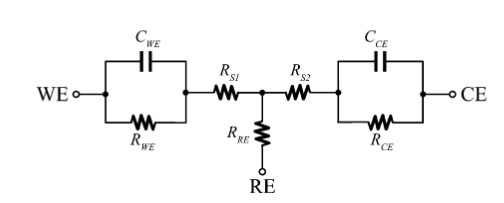
\includegraphics[width=1.\linewidth]{../Media/electricalModel_EC_sensor.PNG}
		\caption{Het elektrisch equivalente model van een elektrochemische gassensor \cite{Mohammad Mahdi Ahmadi}}
		\label{fig::EG_equivalent}
	\end{figure}
	Echter zijn de waardes voor het elektrisch equivalent model van de \textit{3SP\_CO\_1000 package 110-102} niet terug te vinden in de datasheet. Hiervoor is er namens groep 5 een email gestuurd naar fabrikant, echter is hier nog niet op  gereageerd waardoor er helaas geen simulaties uitgevoerd konden worden.
	
	\section{Thermometer} \label{sec::thermometer}
	In dit hoofdstuk wordt er besproken hoe de temperatuur gemeten gaat worden en wat de nodige signaal verwerking is om deze correct uit te kunnen lezen.
	\subsection{NTC thermistor} \label{subsec::NTC_thermistor}
	Voor het meten van de temperatuur is er gekozen om een NTC thermistor te gebruiken. Een thermistor is een type halfgeleider waarbij de temperatuur een groter effect heeft op de weerstandswaarde dan bij "standaard" weerstanden, m.a.w. het heeft een groter (of juist kleiner in het geval van een negatief) temperatuurcoëfficiënt dan "standaardaard" weerstanden \cite{thermistor}.
	\newpage
	\subsubsection{Niet lineair}
	De relatie tussen de weestandwaarde en de temperatuur is bij een NTC thermistor niet lineair, Zie figuur \ref{fig::thermistorCurve}. 
	\begin{figure}[h!]
		\centering
		\hspace*{-1cm} 
		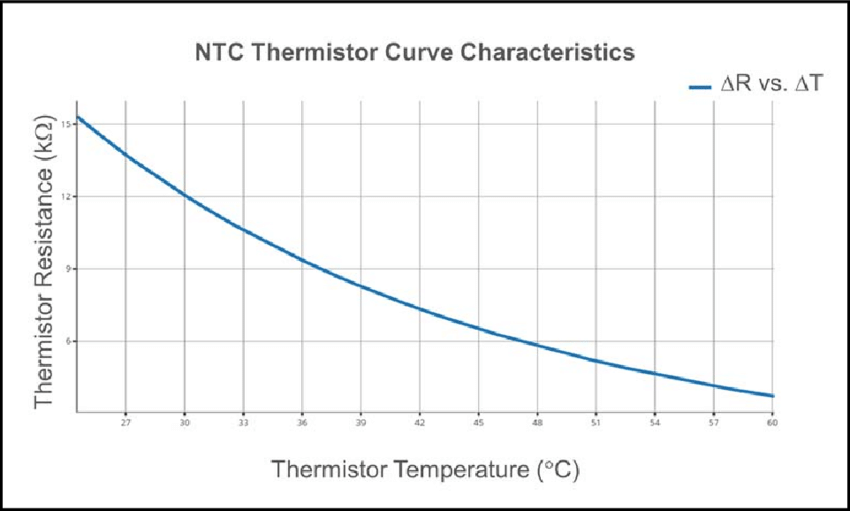
\includegraphics[width=1.2\linewidth]{../Media/thermistorCurve.png}
		\caption{Een karakteristieke curve van een NTC thermistor} \cite{thermistorCurve}
		\label{fig::thermistorCurve}
	\end{figure}
	Deze relatie kan omschreven worden met relatief complexe formules, het is dan ook belangrijk om deze meer lineair te maken om de NTC thermistor te kunnen gebruiken om de temperatuur mee uit te kunne lezen. Door de thermistor parallel te schakelen met een andere weerstand veranderd de curve in een "S-curve" met een omslagpunt. Bij dit omslag punt is deze "S-curve" nagenoeg lineair en kan deze benaderd worden volgens de standaard functie
	\begin{math}
		y = ax + b
	\end{math} \cite{TDK}.
	Zie figuur \ref{fig::s_curve}
	\newpage
	\begin{figure}[h!]
		\centering
		\hspace*{-1cm} 
		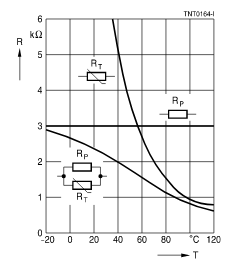
\includegraphics[width=0.7\linewidth]{../Media/lineairNTC.png}
		\caption{karakteristieke "S-curve" van NTC thermistor parallel geschakeld met een weerstand \cite{TDK}} \cite{thermistorCurve}
		\label{fig::s_curve}
	\end{figure}
	Het doel is om het omslagpunt van de "S-curve" bij de gebruikstemperatuur te krijgen, aangezien dit ontwerp zich richt op het gebruik in werkomgevingen zoals kantoren en universiteiten zal de gebruikstemperatuur in dit geval op kamertemperatuur liggen (293 \degree K of 20 \degree C). Om dit te realiseren moet de juiste waarde van weerstand \begin{math} R_p \end{math} gekozen worden. Deze kan op de volgende manier berekend worden:\\
	\begin{center}
		\cite{TDK} \\
		\Large
		\begin{math}
		R_p = R_T \frac{B-2T}{B+2T}
		\end{math}
	\end{center}
	Hierbij is \textit{B} de beta-waarde van de NTC thermistor (temperatuurcoëfficiënt), \textit{R{\small T}} de weerstandswaarde van de NTC thermistor op de gebruikstemperatuur en \textit{T} de temperatuur in \degree K.
	\newpage
	\subsection{Simulaties}
	Om de temperatuur uit te lezen rond de gebruikstemperatuur met een ADC wordt er gebruik gemaakt van een spanningsdeler. zie figuur \ref{fig::thermistor_circ}
	\begin{figure}[h!]
		\centering
		\hspace*{-1cm} 
		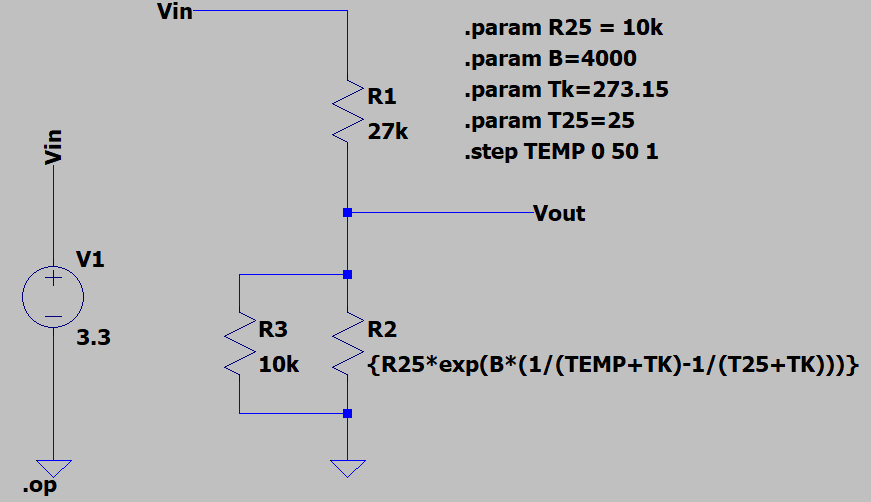
\includegraphics[width=1\linewidth]{../Media/thermistor_circ.PNG}
		\caption{Schakeling voor het uitlezen van de temperatuur d.m.v. een thermistor}
		\label{fig::thermistor_circ}
	\end{figure}
	\begin{figure}[h!]
		\centering
		\hspace*{-1cm} 
		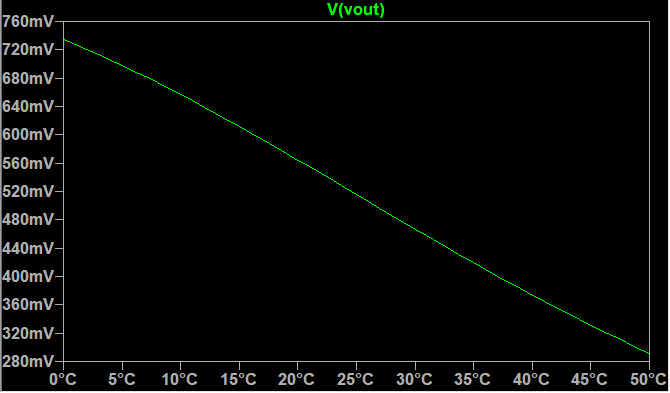
\includegraphics[width=1\linewidth]{../Media/thermistor_sim.PNG}
		\caption{De uitgangsspanning rond de gebruikstemperatuur in relatie tot de temperatuur}
		\label{fig::thermistor_sim}
	\end{figure}
	\newpage
	Vervolgens kan de spanning uitgelezen worden met een ADC. Aangezien deze nagenoeg lineair, kan de temperatuur herleid worden van uit de spanning volgens de formule \begin{math}
	y = ax + b
	\end{math}. Vervolgens kan deze informatie gebruikt worden om de fouten ter gevolgen van de temperatuursverandering van de CO-sensor te compenseren.
	%----------------------------------------------------------------------------------------
	\newpage
	
	\begin{thebibliography}{9}
		\bibitem{datasheet sensor}
		SPEC SENSORS,
		april 2017 [bekeken in november 2019],
		[Datasheet],
		"3SP\_CO\_1000 package 110-102",
		Beschikbaar:
		\url{https://www.spec-sensors.com/wp-content/uploads/2016/04/3SP_CO_1000-P-Package-110-102.pdf}
		
		\bibitem{SGX Application note}
		SGX SENSORTECH,
		juli 2016 [bekeken in november 2019],
		[Application Note],
		"Electrochemical Sensors Application Note 2Design of Electronics for Electrochemical Gas Sensors",
		Beschikbaar:
		\url{https://www.sgxsensortech.com/content/uploads/2014/08/A1A-EC_SENSORS_AN2-Design-of-Electronics-for-EC-Sensors-V4.pdf}
		
		\bibitem{Mohammad Mahdi Ahmadi}
		Mohammad Mahdi Ahmadi,
		juli 2009 [bekeken in december 2019],
		[Artikel],
		"Current-Mirror-Based Potentiostats for Three-Electrode Amperometric Electrochemical Sensors"
		
		\bibitem{thermistor}
		Omega Engineering Inc.,
		augustus 2018 [bekeken in december 2019],
		[Online],
		"What is a Thermistor and how does it work?",
		Beschikbaar:
		\url{https://www.omega.com/en-us/resources/thermistor}	
			
		\bibitem{thermistorCurve}
		februari 2018 [bekeken in december 2019],
		[Online],
		"http://www.giangrandi.ch/electronics/ntc/ntc.shtml",
		Beschikbaar:
		\url{http://www.giangrandi.ch/electronics/ntc/ntc.shtml}	
			
		\bibitem{TDK}
		TDK,
		januari 2018 [bekeken in december 2019],
		[Application Note],
		"NTC thermistors application notes",
		Beschikbaar:
		\url{https://www.tdk-electronics.tdk.com/download/531110/5608e4b12153bb12af2808fbedc5a55b/pdf-applicationnotes.pdf}

	\end{thebibliography}
\end{document}
